\chapter{Vorgehen Performanceanalyse}
\section{Motivation}

Die Performance respektive Leistungsfähigkeit einer Applikation stellt einer der bedeutendsten Qualitätsanforderungen dar. Sie kann nich nur zu verärgerten Benutzern, sondern auch zu einer Verlangsamung der Business-Prozesse führen. Die Motivation für eine Performanceanalyse entsteht, wenn die in Service Level Agreement oder Anforderungsanalyse spezifizierten \textbf{Qualitätsanforderungen nicht erfüllt} sind. Optimal wäre, wenn diese Anforderung während des Entwicklungsprozesses kontinuierlich geprüft würde.

\section{Ablauf}
Die Performanceanalyse ist ein iterativer Prozess und sollte so lange dauern, bis die Anforderungen erfüllt und der Kunde zufrieden ist. Sie besteht aus folgenden vier Schritten\cite{hummelBeer201109}:
\begin{enumerate}
	\item Identifikation der neuralgischen Punkte des Systems
	\item \textbf{Suche nach dem Dominating Consumer\footnote{Kirk Pepperdine bezeichnet die Aktivität, welche dominiert wie die CPU gebraucht wird, als Dominating Consumer . } (Abschnitt \ref{dominating_consumer})}
	\item \textbf{Sammeln von Detaildaten (Abschnitt \ref{garbage_collection_tuning})}
	\item Lösen des Problems
\end{enumerate}


Damit die Analyse der Garbage Collection zum richtigen Zeitpunkt gemacht wird, sind insbesondere die Punkte zwei und drei wichtig. Sie werden in den folgenden beiden Abschnitten genauer definiert.
\section{Suche nach dem Dominating Consumer}\label{dominating_consumer}
Die Suche nach dem Dominating Consumer kann nach folgendem Schema durchgeführt werden:
\begin{figure}[H]
  	\centering
    	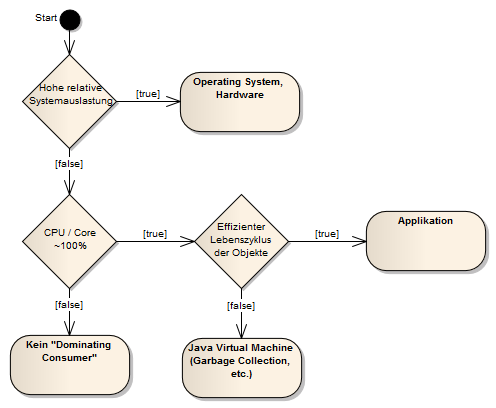
\includegraphics[width=13.1cm]{images/dominating_consumer}
        	\caption{Suche nach dem Dominating Consumer}
\end{figure}

\subsection{Hohe relative Systemlast}\label{hohe_systemauslastung}
Die erste Frage, die sich bei der Suche nach dem Dominating Consumer stellt, ist, ob die hohe CPU-Auslastung\footnote{CPU kann auch einer oder ein paar Cores bedeuten.} durch die Applikation oder das System verursacht wird. Je nach Betriebssystemen gibt es dafür unterschiedliche Werkzeuge:
\begin{itemize}
	\item \textbf{Windows:} Task Manager / Lasche Performance (Leistung). Für die Anzeige der Systemzeit muss die Anzeige der Kernelzeit eingeblendet werden: View / Show Kernel Times
	\item \textbf{Linux / Unix: } vmstat zeigt die Ausnutzung der CPU: vmstat 5
\end{itemize}

Hohe Systemauslastung kann unterschiedliche Gründe haben: 
\begin{itemize}
\item \textbf{Exzessives Context-Switching\footnote{Kontextwechsel}:} Mehrere Prozesse können sich die gleiche CPU (CPU-Kern) nur deshalb teilen, weil beim Wechsel von Prozess A auf B ein Context-Switch gemacht wird, so dass Thread B am selben Ort weiterarbeitet wo er beim letzten Mal war. Gründe für exzessives Context-Switching können beispielsweise nicht adäquat gewählte Locks sein. Wenn ein Thread aufgrund der Synchronisation angehalten werden muss.\footnote{Symptomatisch zeigt dann vmstat, das System ist nicht im Leerlauf, aber die Kernelzeiten (cpu/sy) dominieren die Zeit des Benutzers (cpu/us).}
\item \textbf{Hohe I/O Festplatte} 
\item \textbf{Hohe I/O Netzwerk} 
\end{itemize}


\subsection{Hohe CPU- respektive Core-Last}
Sofern die im Abschnitt \ref{hohe_systemauslastung} beschriebenen Punkte nicht zutreffen, stellt sich die Frage, ob die Auslastung der CPU überhaupt gross ist. Ist das nicht der Fall, gibt es womöglich gar keinen Dominating Consumer - es muss dann herausgefunden werden, was die Threads weg von der CPU haltet. Es gibt dafür laut \cite{pepperdine201102} unterschiedliche Gründe:
\begin{itemize}
\item \textbf{Dead Locks: } Threads schliessen sich gegenseitig aus. 
\item \textbf{Applikation skaliert nicht: } Applikation hat schlechte multi-core Eigenschaften.
\item \textbf{Langsame Disks / Netzwerke}
\item \textbf{Zu kleine Connection- und Thread-Pools}
\item \textbf{Aurufe auf langsame externe Systeme}
\end{itemize}


\subsection{Effizienter Objekt-Lebenszyklus}
Sofern die relative Systemlast klein und die CPU-Auslastung gross ist, muss der Lebenszyklus der Objekte angeschaut werden. Dies kann auf unterschiedliche Arten getan werden:
\begin{itemize}
\item \textbf{Memory Analyse: }Es wird angeschaut, wie alt die Objekte in den verschiedenen Bereiche (Young Collection, Old Collection) sind. Wieviele Garbage Collection Zyklen sie überlebt haben.
\item \textbf{Garbage Collection: }Wann und wie oft werden Garbage Collections durchgeführt, wie lange haben sie gedauert, wieviel Speicher haben sie befreit.
\end{itemize}

\section{Garbage Collection Tuning}\label{garbage_collection_tuning}
Mit der Analyse des Dominating Consumers entscheidet sich auch, in welchem Bereich anschliessend weitere Detaildaten gesammelt werden. Auch beim Garbage Collection Tuning gilt grundsätzlich: "never change a running system". Man ändert also nur etwas, wenn es Probleme bei der Garbage Collection respektive die Anforderungen daran nicht erfüllt sind. Mit dem Tuning will man in der Regel drei unterschiedliche Ziele erreichen\cite{langerkreftJavaCore}: 
\begin{itemize}
\item Verbesserung des Durchsatzes (siehe Abschnitt \ref{gc_tuning_durchsatz})
\item Geringere Pausenzeiten (siehe Abschnitt \ref{gc_tuning_pausenzeiten})
\item Geringerer Speicherverbrauch (siehe Abschnitt \ref{gc_tuning_speicherverbrauch})
\end{itemize}

Diese drei Ziele bilden eine Dreiecksbeziehung, zum Beispiel führt eine aggressive Optimierung des Durchsatzes in der Regel zu längeren Stop-the-World\footnote{Zeiten in welchen die Prozessoren der Anwendung keine Rechenzeiten zur Verfügung stellen.} Pausen. Tuning bedeutet nun, zwei der Ziele konstant halten, während das dritte durch Anpassung der Konfiguration verbessert wird. Sofern die Optimierung nicht ausreicht, müssen einer oder beide anderen Parameter aufgegeben werden, um das Ziel zu erreichen.


\subsection{Durchsatz\label{gc_tuning_durchsatz}}
Die relative Zeit der CPU welcher der Anwendung zur Verfügung steht nennt man Durchsatz (englisch \textit{Throughput}). Es handelt sich also um einen Prozentsatz im Vergleich mit der gesamten CPU-Zeit. Grundsätzlich ist wird der Durchsatz folgendermassen ausgerechnet:

 \begin{align*}
         Durchsatz &= 100 * (1-Relative\;Zeit\;in\;Garbage\;Collection)\\
         Durchsatz &= 100 * (1-\frac{Zeit\;in\;Garbage\;Collection}{Gesamtdauer\;der\;Messung})
 \end{align*}
Im Prinzip ist diese Formel ziemlich ungenau und berücksichtigt nur die Garbage Collection Zeiten während einer Stop-the-World Pause. Insofern ist sie nur für eine Single-Core CPU genau. Bei einer Multi-Core-Maschine müsste der Througput für jeden einzelnen Core ausgewertet und damit der Gesamt-Throughput berechnet werden.\newline

Durchsatz-Tuning spielt in der Praxis oft nur eine untergeordnete Rolle\cite{langerkreftJavaCore}. Eine wirkliche Steigerung des Durchsatzes kann man nur mit einer aggressiven Optimierung erzielen, sie führt zu verlängerten Pausenzeiten, was nur bei Batch-Applikationen toleriert werden kann. Gleichzeitig ist der Austausch oder das Zuschalten von weiteren CPUs sehr rasch der kostengünstigere Weg.

\subsection{Pausenzeiten\label{gc_tuning_pausenzeiten}}
In der Regel geht es beim Garbage Collection Tuning um das Tuning der Pausenzeiten, dies weil man die Symptome wie Stottern und einer ungleich reaktionsfreudigen Anwendung beseitigen möchte. 

In der Regel startet man mit der Analyse einzelner Garbage Collections. Die Gründe für die Initiierung einer Garbage Collection können sehr unterschiedlich sein und müssen entsprechend behandelt werden:
\begin{itemize}
\item \textbf{Erreichen eines Schwellenwerts des Young- oder Old-Spaces: } Anpassung der Grösse des Young- / Old-Spaces, Vergrösserung des Heaps, etc.
\item \textbf{Heap hat maximale Grösse erreicht:} Anpassung der Heap-Grösse, Beseitigung von Memory Leaks, etc.
\item \textbf{Allokation von Objekten ist nicht möglich:} Vergrösserung des Young-Space, Beseitung der Fragmentierung, etc. 
\item \textbf{Von der Applikation innitiert (System.gc()):} Von der Applikation ausgelöste Garbage Collections können mittels einem Flag ignoriert werden.
\end{itemize}



\subsection{Speicherverbrauch\label{gc_tuning_speicherverbrauch}}
Dieses Tuningziel verliert insofern an relevanz, weil 64-Bit-JVMs bei grossen Applikationen schon sehr verbreitet sind. Mit den 32-Bit Adressen kam man im Bereich des Arbeitsspeichers schon eher an die Grenze (ein Teil des adressierbaren Bereichs von 4GB bei 32-Bit-Adressen wird auch noch Für das Betriebssystem verwendet). Eine Optimierung im Bereich des Speicherverbrauchs hat in der Regel nichts mit Garbage Collection Tuning zu tun, sondern ist eine Analyse der Objektpopulation im Bereich der Applikation.

